\documentclass{standalone}
\usepackage{tikz}
\usetikzlibrary{patterns, positioning}


\begin{document}
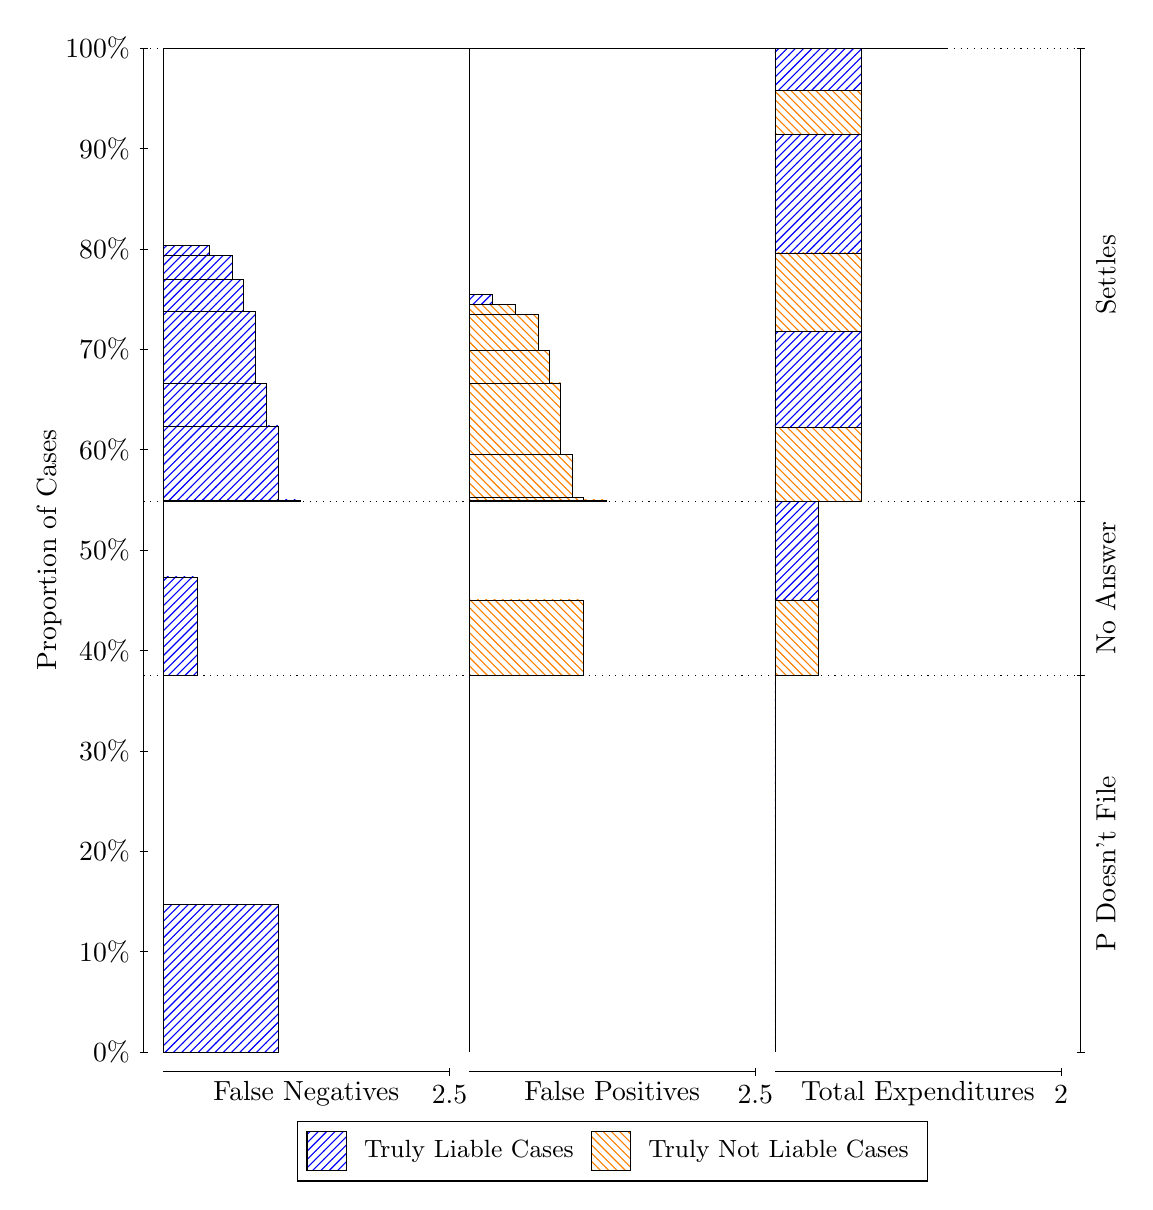
\begin{tikzpicture}
\draw[black, very thin] (1.5,1.75) -- (1.5,14.5);
\node[rotate=90, text=black, anchor=center] at (0.3, 8.125) {Proportion of Cases};
\draw[black, very thin] (1.45,1.75) -- (1.55,1.75);
\node[text=black, anchor=east] at (1.45, 1.75) {0\%};
\draw[black, very thin] (1.45,3.025) -- (1.55,3.025);
\node[text=black, anchor=east] at (1.45, 3.025) {10\%};
\draw[black, very thin] (1.45,4.3) -- (1.55,4.3);
\node[text=black, anchor=east] at (1.45, 4.3) {20\%};
\draw[black, very thin] (1.45,5.575) -- (1.55,5.575);
\node[text=black, anchor=east] at (1.45, 5.575) {30\%};
\draw[black, very thin] (1.45,6.85) -- (1.55,6.85);
\node[text=black, anchor=east] at (1.45, 6.85) {40\%};
\draw[black, very thin] (1.45,8.125) -- (1.55,8.125);
\node[text=black, anchor=east] at (1.45, 8.125) {50\%};
\draw[black, very thin] (1.45,9.4) -- (1.55,9.4);
\node[text=black, anchor=east] at (1.45, 9.4) {60\%};
\draw[black, very thin] (1.45,10.675) -- (1.55,10.675);
\node[text=black, anchor=east] at (1.45, 10.675) {70\%};
\draw[black, very thin] (1.45,11.95) -- (1.55,11.95);
\node[text=black, anchor=east] at (1.45, 11.95) {80\%};
\draw[black, very thin] (1.45,13.225) -- (1.55,13.225);
\node[text=black, anchor=east] at (1.45, 13.225) {90\%};
\draw[black, very thin] (1.45,14.5) -- (1.55,14.5);
\node[text=black, anchor=east] at (1.45, 14.5) {100\%};

\draw[black, very thin] (13.4,1.75) -- (13.4,14.5);
\draw[black, very thin] (13.35,1.75) -- (13.45,1.75);
\node[anchor=west] at (13.35, 1.75) {};
\draw[black, very thin] (13.35,6.5345) -- (13.45,6.5345);
\node[anchor=west] at (13.35, 6.5345) {};
\draw[black, very thin] (13.35,8.7413) -- (13.45,8.7413);
\node[anchor=west] at (13.35, 8.7413) {};
\draw[black, very thin] (13.35,14.496) -- (13.45,14.496);
\node[anchor=west] at (13.35, 14.496) {};
\draw[black, very thin] (13.35,14.498) -- (13.45,14.498);
\node[anchor=west] at (13.35, 14.498) {};
\draw[black, very thin] (13.35,14.5) -- (13.45,14.5);
\node[anchor=west] at (13.35, 14.5) {};

\draw[black, very thin, pattern color=blue, pattern=north east lines] (1.75,1.75) rectangle (3.2033,3.6243);
\draw[black, very thin, pattern color=orange, pattern=north west lines] (1.75,3.6243) rectangle (1.75,6.5345);
\draw[black, very thin, pattern color=blue, pattern=north east lines] (1.75,6.5345) rectangle (2.186,7.7842);
\draw[black, very thin, pattern color=orange, pattern=north west lines] (1.75,7.7842) rectangle (1.75,8.7413);
\draw[black, very thin, pattern color=blue, pattern=north east lines] (1.75,8.7413) rectangle (3.494,8.7614);
\draw[black, very thin, pattern color=blue, pattern=north east lines] (1.75,8.7614) rectangle (3.2033,9.7001);
\draw[black, very thin, pattern color=blue, pattern=north east lines] (1.75,9.7001) rectangle (3.058,10.241);
\draw[black, very thin, pattern color=blue, pattern=north east lines] (1.75,10.241) rectangle (2.9127,11.152);
\draw[black, very thin, pattern color=blue, pattern=north east lines] (1.75,11.152) rectangle (2.7673,11.561);
\draw[black, very thin, pattern color=blue, pattern=north east lines] (1.75,11.561) rectangle (2.622,11.863);
\draw[black, very thin, pattern color=blue, pattern=north east lines] (1.75,11.863) rectangle (2.3313,11.99);
\draw[black, very thin, pattern color=orange, pattern=north west lines] (1.75,11.99) rectangle (1.75,14.496);
\draw[black, very thin, pattern color=blue, pattern=north east lines] (1.75,14.496) rectangle (5.8193,14.497);
\draw[black, very thin, pattern color=orange, pattern=north west lines] (1.75,14.497) rectangle (1.75,14.498);
\draw[black, very thin, pattern color=orange, pattern=north west lines] (1.75,14.498) rectangle (1.75,14.499);
\draw[black, very thin, pattern color=blue, pattern=north east lines] (1.75,14.499) rectangle (1.75,14.5);
\draw[black, very thin, pattern color=orange, pattern=north west lines] (5.6333,1.75) rectangle (5.6333,4.6602);
\draw[black, very thin, pattern color=blue, pattern=north east lines] (5.6333,4.6602) rectangle (5.6333,6.5345);
\draw[black, very thin, pattern color=orange, pattern=north west lines] (5.6333,6.5345) rectangle (7.0867,7.4916);
\draw[black, very thin, pattern color=blue, pattern=north east lines] (5.6333,7.4916) rectangle (5.6333,8.7413);
\draw[black, very thin, pattern color=orange, pattern=north west lines] (5.6333,8.7413) rectangle (7.3773,8.7614);
\draw[black, very thin, pattern color=orange, pattern=north west lines] (5.6333,8.7614) rectangle (7.0867,8.796);
\draw[black, very thin, pattern color=orange, pattern=north west lines] (5.6333,8.796) rectangle (6.9413,9.337);
\draw[black, very thin, pattern color=orange, pattern=north west lines] (5.6333,9.337) rectangle (6.796,10.248);
\draw[black, very thin, pattern color=orange, pattern=north west lines] (5.6333,10.248) rectangle (6.6507,10.657);
\draw[black, very thin, pattern color=orange, pattern=north west lines] (5.6333,10.657) rectangle (6.5053,11.12);
\draw[black, very thin, pattern color=orange, pattern=north west lines] (5.6333,11.12) rectangle (6.2147,11.247);
\draw[black, very thin, pattern color=blue, pattern=north east lines] (5.6333,11.247) rectangle (5.924,11.374);
\draw[black, very thin, pattern color=blue, pattern=north east lines] (5.6333,11.374) rectangle (5.6333,14.496);
\draw[black, very thin, pattern color=orange, pattern=north west lines] (5.6333,14.496) rectangle (5.6333,14.497);
\draw[black, very thin, pattern color=blue, pattern=north east lines] (5.6333,14.497) rectangle (5.6333,14.498);
\draw[black, very thin, pattern color=orange, pattern=north west lines] (5.6333,14.498) rectangle (9.7027,14.499);
\draw[black, very thin, pattern color=blue, pattern=north east lines] (5.6333,14.499) rectangle (8.2493,14.5);
\draw[black, very thin, pattern color=orange, pattern=north west lines] (9.5167,1.75) rectangle (9.5167,4.6602);
\draw[black, very thin, pattern color=blue, pattern=north east lines] (9.5167,4.6602) rectangle (9.5167,6.5345);
\draw[black, very thin, pattern color=orange, pattern=north west lines] (9.5167,6.5345) rectangle (10.062,7.4916);
\draw[black, very thin, pattern color=blue, pattern=north east lines] (9.5167,7.4916) rectangle (10.062,8.7413);
\draw[black, very thin, pattern color=orange, pattern=north west lines] (9.5167,8.7413) rectangle (10.607,9.6866);
\draw[black, very thin, pattern color=blue, pattern=north east lines] (9.5167,9.6866) rectangle (10.607,10.899);
\draw[black, very thin, pattern color=orange, pattern=north west lines] (9.5167,10.899) rectangle (10.607,11.899);
\draw[black, very thin, pattern color=blue, pattern=north east lines] (9.5167,11.899) rectangle (10.607,13.399);
\draw[black, very thin, pattern color=orange, pattern=north west lines] (9.5167,13.399) rectangle (10.607,13.96);
\draw[black, very thin, pattern color=blue, pattern=north east lines] (9.5167,13.96) rectangle (10.607,14.496);
\draw[black, very thin, pattern color=orange, pattern=north west lines] (9.5167,14.496) rectangle (11.697,14.497);
\draw[black, very thin, pattern color=blue, pattern=north east lines] (9.5167,14.497) rectangle (11.697,14.498);
\draw[black, very thin, pattern color=orange, pattern=north west lines] (9.5167,14.498) rectangle (11.697,14.499);
\draw[black, very thin, pattern color=blue, pattern=north east lines] (9.5167,14.499) rectangle (11.697,14.5);
\draw[black, dotted] (1.5,6.5345) -- (13.4,6.5345);
\draw[black, dotted] (1.5,8.7413) -- (13.4,8.7413);
\draw[black, dotted] (1.5,14.496) -- (13.4,14.496);
\draw[black, dotted] (1.5,14.498) -- (13.4,14.498);
\draw[black, very thin] (1.75,1.5) -- (5.3833,1.5);
\node[text=black, anchor=north] at (3.5667, 1.5) {False Negatives};
\draw[black, very thin] (5.3833,1.45) -- (5.3833,1.55);
\node[text=black, anchor=north] at (5.3833, 1.45) {2.5};

\draw[black, very thin] (5.6333,1.5) -- (9.2667,1.5);
\node[text=black, anchor=north] at (7.45, 1.5) {False Positives};
\draw[black, very thin] (9.2667,1.45) -- (9.2667,1.55);
\node[text=black, anchor=north] at (9.2667, 1.45) {2.5};

\draw[black, very thin] (9.5167,1.5) -- (13.15,1.5);
\node[text=black, anchor=north] at (11.333, 1.5) {Total Expenditures};
\draw[black, very thin] (13.15,1.45) -- (13.15,1.55);
\node[text=black, anchor=north] at (13.15, 1.45) {2};

\node[text=black, centered, rotate=90] at (13.72, 4.1423) {P Doesn't File};
\node[text=black, centered, rotate=90] at (13.72, 7.6379) {No Answer};
\node[text=black, centered, rotate=90] at (13.72, 11.619) {Settles};



\draw (7.449999999999999,1.5) node[draw=none] (baseCoordinate) {};
\begin{scope}[align=center]
        \matrix[scale=0.5, draw=black, below=0.5cm of baseCoordinate, nodes={draw}, column sep=0.1cm]{
            \node[rectangle, draw, minimum width=0.5cm, minimum height=0.5cm, pattern color=blue, pattern=north east lines] {}; &
            \node[draw=none, font=\small, text=black] (B) {Truly Liable Cases}; &
            \node[rectangle, draw, minimum width=0.5cm, minimum height=0.5cm, pattern color=orange, pattern=north west lines] {}; &
            \node[draw=none, font=\small, text=black] (B) {Truly Not Liable Cases}; \\
            };
\end{scope}

\end{tikzpicture}
\end{document}